%\documentclass{sig-alternate-05-2015}
\documentclass{llncs}
\usepackage{makeidx}
\usepackage{tabularx,colortbl}
\usepackage[dvipsnames]{xcolor}
\usepackage{flushend}
\usepackage{cite}
\usepackage{amsmath}
%\usepackage{amsthm}
\usepackage{amssymb}
\usepackage{epsfig}
\usepackage{stmaryrd}
\usepackage{url}
\usepackage{multirow}
\usepackage{latexsym}
\usepackage{graphics}
\usepackage{graphicx}
\usepackage{enumitem}
\usepackage{comment}
\usepackage{longtable}
\usepackage{supertabular}
\usepackage{times}
\usepackage{listings}
\usepackage{subfigure}
\usepackage{color}
\usepackage{balance}
\usepackage{xspace}
\usepackage[ruled, vlined, linesnumbered]{algorithm2e}
\usepackage[autostyle]{csquotes}



%\theoremstyle{Definition}
%\newtheorem{definition}{Definition}
%%%
%\theoremstyle{Theorem}
%\newtheorem{theorem}{Theorem}


%\newcommand{\definition}{\noindent \textbf{Definition} \citation{}}
%\newcommand{\theorem}{\noindent \textbf{Theorem} \citation{}}
%\newcommand{\lemma}{\noindent \textbf{Lemma} \citation{}}

%\newdef{lemma}{Lemma}
%\newdef{definition}{Definition}
%\newdef{theorem}{Theorem}
%\newdef{corollary}{Corollary}
%\newdef{note}{Note}
%\newdef{axiom}{Axiom}
\newcommand{\mkeyword}[1]{\mbox{\texttt{#1}}}
\DeclareMathOperator{\kuop}{uop}
\DeclareMathOperator{\kbop}{bop}
\DeclareMathOperator{\kite}{ite}
\DeclareMathOperator{\kpre}{pre}
\DeclareMathOperator{\dom}{dom}
\DeclareMathOperator{\ktrue}{true}
\DeclareMathOperator{\kfalse}{false}
\DeclareMathOperator{\kselect}{select}
\DeclareMathOperator{\ran}{range}
\newcommand{\lbb}{[\![}
\newcommand{\rbb}{]\!]}
\newcommand{\expr}{\phi}
\newcommand{\exprS}{\Phi}
\newcommand{\mike}[1]{\textcolor{red}{#1}}
\newcommand{\mats}[1]{\textcolor{blue}{#1}}
\newcommand{\darren}[1]{\textcolor{green}{#1}}
\newcommand{\danielle}[1]{\textcolor{orange}{#1}}

\sloppypar



\begin{document}

\definecolor{gold}{rgb}{0.90,.66,0}
\definecolor{dgreen}{rgb}{0,0.6,0}
\newcommand{\stateequiv}{\equiv_{s}}
\newcommand{\traceequiv}{\equiv_{\sigma}}
\newcommand{\ta}{\text{TA}}
\newcommand{\cta}{\text{TA$_{C}$}}
\newcommand{\tta}{\text{TA$_{T}$}}
\newcommand{\ucalg}{\texttt{\small{IVC\_UC}}}
\newcommand{\ucbfalg}{\texttt{\small{IVC\_UCBF}}}


\title{Architectural Modeling and Analysis for Safety Engineering}
%
\author{Danielle Stewart\inst{1}
\and Michael W. Whalen\inst{1}
\and Darren Cofer\inst{2}
\and Mats P.E. Heimdahl\inst{1} }
\institute{University of Minnesota\\Department of Computer
Science and Engineering\\
200 Union Street\\
Minneapolis, MN, 55455, USA\\
\email{whalen, dkstewar, heimdahl@cs.umn.edu}
\and
Rockwell Collins\\
Advanced Technology Center\\400 Collins Rd. NE\\
Cedar Rapids, IA, 52498, USA\\ \email{ darren.cofer@rockwellcollins.com}
}
\maketitle

\begin{abstract}
Architecture description languages such as AADL allow systems engineers to specify the structure of system architectures and perform several analyses over them, including schedulability, resource analysis, and information flow.  In addition, they
permit system-level requirements to be specified and analyzed early in the development process of airborne and ground-based systems. These tools can also be used to perform safety analysis based on the system architecture and initial functional decomposition.

%Previously, Rockwell Collins and the University of Minnesota developed and demonstrated an approach to behavioral model-based safety analysis using Simulink. New MBSE tools that incorporate assume-guarantee compositional analysis techniques provide the basis for greatly improving earlier approaches to safety analysis and can be used to ensure model consistency, correctness of assumptions, and better scalability.

Using AADL-based system architecture modeling and analysis tools as an exemplar, we extend existing analysis methods to support system safety objectives of ARP4754A and ARP4761. This includes extensions to existing modeling languages to better describe failure conditions, interactions, and mitigations, and improvements to compositional reasoning approaches focused on the specific needs of system safety analysis. We develop example systems based on the Wheel Braking System in SAE AIR6110 to evaluate the effectiveness and practicality of our approach.
\end{abstract}

\keywords{Model-based systems engineering, fault analysis, safety engineering}

\section{Introduction}
\label{sec:intro}

%This paper describes a new methodology with tool support for model based safety analysis. It is implemented as a {\em Safety Annex} for the Architecture Analysis and Design Language (AADL). The Safety Annex provides the ability to describe faults and faulty component behaviors in AADL models. In contrast to previous AADL-based approaches, the Safety Annex leverages a formal description of the nominal system behavior to propagate faults in the system. This approach ensures consistency with the rest of the system development process and simplifies the work of safety engineers. The language for describing faults is extensible and allows safety engineers to weave various types of faults into the nominal system model. The Safety Annex supports the injection of faults into component level outputs, and the resulting behavior of the system can be analyzed using model checking through the Assume-Guarantee Reasoning Environment (AGREE).

System safety analysis techniques are well-established and are a required activity in the development of safety-critical systems. Model-based systems engineering (MBSE) methods and tools based on formal methods now permit system-level requirements to be specified and analyzed early in the development process~\cite{NFM2012:CoGaMiWhLaLu,CAV2015:BoCiGrMa}. While model-based development methods are widely used in the aerospace industry, they are only recently being applied to system safety analysis.  

%How can we leverage these model-based methods and tools to perform safety analysis based on models of the system architecture and initial functional decomposition? Can these design models be integrated into the safety analysis process to help guarantee accurate and consistent results?
%Seeking solutions to these questions are especially important as the amount of safety-critical hardware and software in various domains has drastically increased due to the demand for greater autonomy, capability, and connectedness.

In this paper, we describe a {\em Safety Annex} for the Architecture Analysis and Design Language (AADL)~\cite{FeilerModelBasedEngineering2012} that provides the ability to reason about faults and faulty component behaviors in AADL models. In the Safety Annex approach, we use formal assume-guarantee contracts to define the nominal behavior of system components. The nominal model is then verified using the Assume Guarantee Reasoning Environment (AGREE)~\cite{NFM2012:CoGaMiWhLaLu}. The Safety Annex  provides a way to weave faults into the nominal system model and analyze the behavior of the system in the presence of faults. The Safety Annex also provides a library of common fault node definitions that is customizable to the needs of system and safety engineers. Our approach adapts the work of Joshi et. al in
~\cite{Joshi05:Dasc} to the AADL modeling language, and provides a domain specific language for the kinds of analysis performed manually in previous work~\cite{Stewart17:IMBSA}.  %More information on the approach is available in~\cite{Stewart17:IMBSA}, and the tool and relevant documentation can be found at: \small \url{https://github.com/loonwerks/AMASE/}. \normalsize

There are other tools purpose-built for safety analysis, including AltaRica~\cite{PROSVIRNOVA2013127}, smartIFlow~\cite{info8010007} and xSAP~\cite{DBLP:conf/tacas/BittnerBCCGGMMZ16}. These notations are separate from the system development model. Other tools extend existing system models, such as HiP-HOPS~\cite{CHEN201391} and the AADL Error Model Annex, Version 2 (EMV2)~\cite{EMV2}. EMV2 uses enumeration of faults in each component and explicit propagation of faulty behavior to perform safety analysis. The required propagation relationships must be manually added to the system model and can become complex, leading to potential omissions and inconsistencies.

In contrast, the Safety Annex supports model checking and quantitative reasoning by attaching behavioral faults to components and then using the normal behavioral propagation and proof mechanisms built into the AGREE AADL annex. This allows users to reason about the evolution of faults over time, and produce counterexamples demonstrating how component faults lead to system failures. It can serve as the shared model to capture system design and safety-relevant information, and produce both qualitative and quantitative description of the causal relationship between faults/failures and system safety requirements.
%
Thus, the contributions of the Safety Annex and this paper are:
\begin{itemize}
\item Close integration of behavioral fault analysis into an {\em architectural design language} AADL, which allows close connection between system and safety analysis and system generation from the model (unlike AltaRica, smartIFlow, and xSAP),
\item support for {\em behavioral specification of faults} and their {\em implicit propagation} through behavioral relationships in the model, in contrast to existing AADL-based annexes (HiP-HOPS and EMV2),
\item additional support for {\em explicit} propagation of faults to capture binding relationships between hardware and software and logical and physical communications beyond what is supported in xSAP, and
\item guidance on integration into a traditional safety analysis process.
\end{itemize}
%\mike{What are our contributions?}


%\section{Safety Assessment Process}
\label{sec:process}
%\mike{COMPLETELY STOLEN FROM THE SAFECOMP-05 PAPER!  Either note it or modify it}
%\danielle{I added a citation. I think this late in the game we might as well just cite it.}

The overall safety assessment process that is followed in practice
in the avionics industry is described in the SAE standard ARP
4761~\cite{SAE:ARP4761}. This section is a summarization of portions of the ARP 47-61 document (also found in~\cite{Joshi05:SafeComp}). 

\iffalse

This section describes the overall safety assessment process that is followed in
practice in the avionics industry along the lines of the SAE standard ARP 47-61 \cite{SAE:ARP4761}. The descriptions of the various phases of the safety assessment process
covered in this section are essentially based on the ARP 47-61 document.

\fi


\begin{figure}
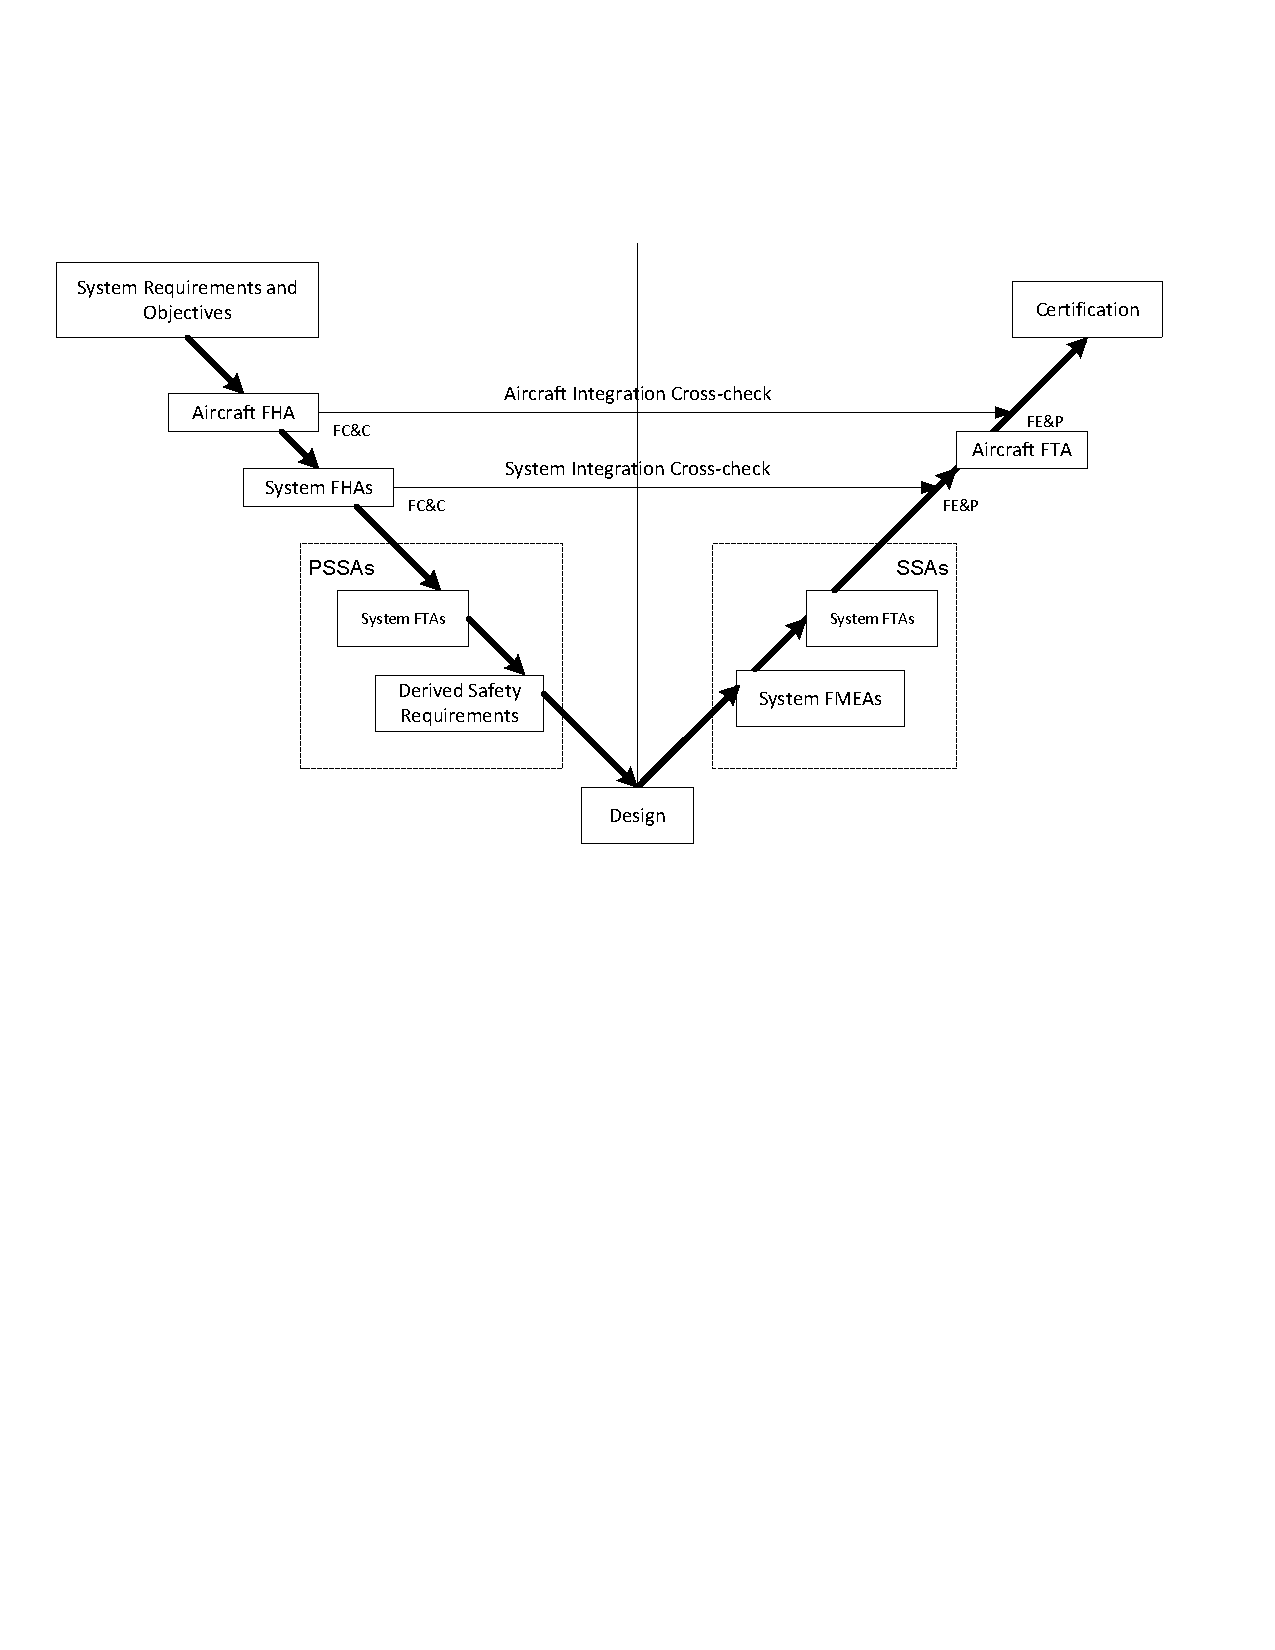
\includegraphics[trim=25 375 0 125, clip, scale=.60]{V}
\caption{Traditional ``V'' Safety Assessment Process} \label{fig:V}
\end{figure}

%The safety assessment process is an integral part of the development process.

Figure~\ref{fig:V} shows an overview of the safety assessment
process as recommended in ARP 4761. The process includes safety
requirements identification (the left side of the ``V'' diagram)
and verification (the right side of the ``V'' diagram), that
support the aircraft development activities. An aircraft level
Functional Hazard Analysis (FHA) is conducted at the beginning of
the aircraft development cycle, which is then followed by system
level FHA for individual sub-systems. The FHA is followed by
Preliminary System Safety Assessment (PSSA), which derives safety
requirements for the subsystems, primarily using Fault Tree
Analysis (FTA). The PSSA process iterates with the design
evolution, with design changes necessitating changes to the
derived system requirements (and also to the fault trees) and
potential safety problems identified through the PSSA leading to
design changes. Once design and implementation are completed, the
System Safety Assessment (SSA) process verifies whether the safety
requirements are met in the implemented design. The system Failure
Modes and Effects Analysis (FMEA) is performed to compute the
actual failure probabilities on the items. The verification is
then completed through quantitative and qualitative analysis of
the fault trees created for the implemented design, first for the
subsystems and then for the integrated aircraft.

%\medskip

We propose to modify this traditional ``V'' process so that the
lower level PSSA and SSA activities are performed based on a
formal model of the system under consideration.
Figure~\ref{fig:Vmod} shows the modified ``V'' diagram for
model-based safety analysis. The shaded blocks are those
activities that will be modified or added.

\begin{figure}
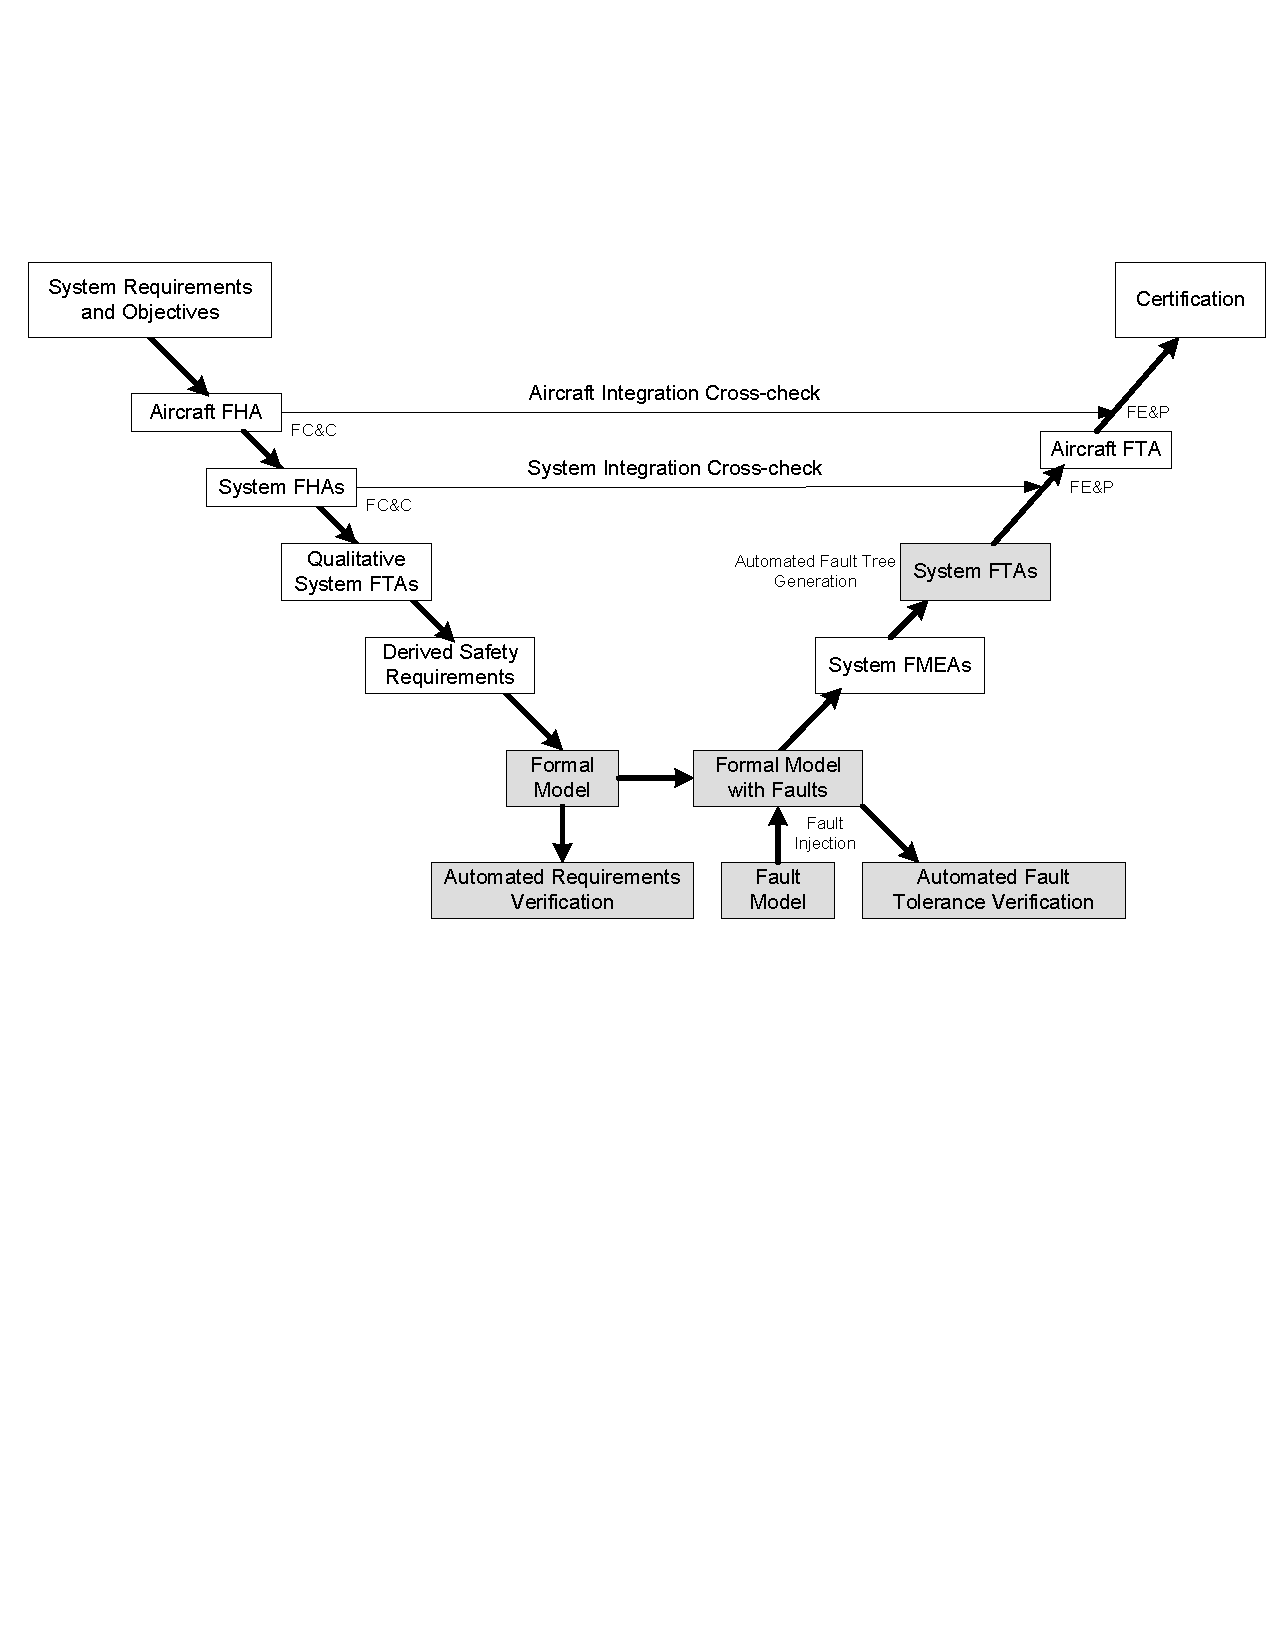
\includegraphics[trim=15 350 0 125, clip, scale=.60]{Mod_V_Process_FaultModel}
\caption{Modified ``V'' Safety Assessment Process} \label{fig:Vmod}
\end{figure}


As we can observe from Figure~\ref{fig:Vmod}, the parts of the analysis that are
primarily affected are at the bottom of the ``V''. The biggest difference is that
the safety analysis activities at this level are now focused around a formal
model of the system behavior, and that many of the artifacts of the safety
analysis can be derived from this model. The idea is to try to pose the right
verification questions to formal tools (such as model checkers and theorem
provers) so that it is possible to derive the necessary safety analysis
information. We then wish to turn the results of these analyses back into
artifacts that can be easily understood and used by safety engineers.


\section{Example: Wheel Brake System}

%\mike{Move the generic description to a section right after the ``safety'' section along with the ARP figure.  Leave the modeling that we did in AADL here.  That way we can reference it in the MBSA sections.}
%\danielle{The whole nominal model description is here. The modeling we did is in the faults section.}

As a preliminary case study, we utilized the Wheel Brake System (WBS) described in \cite{AIR6110} (previously found in ARP4761 Appendix L). This ficticious aircraft system was developed to illustrate the design and safety analysis principles of ARP4754A and ARP4761.  The WBS is installed on the two main aircraft landing gears and is used during taxi, landing, and rejected take off. Braking is either commanded manually using brake pedals or automatically by a digital control system with no need for the pedals (autobrake). When the wheels have traction, the autobrake function will provide a constant smooth deceleration.

\begin{figure}
\begin{center}
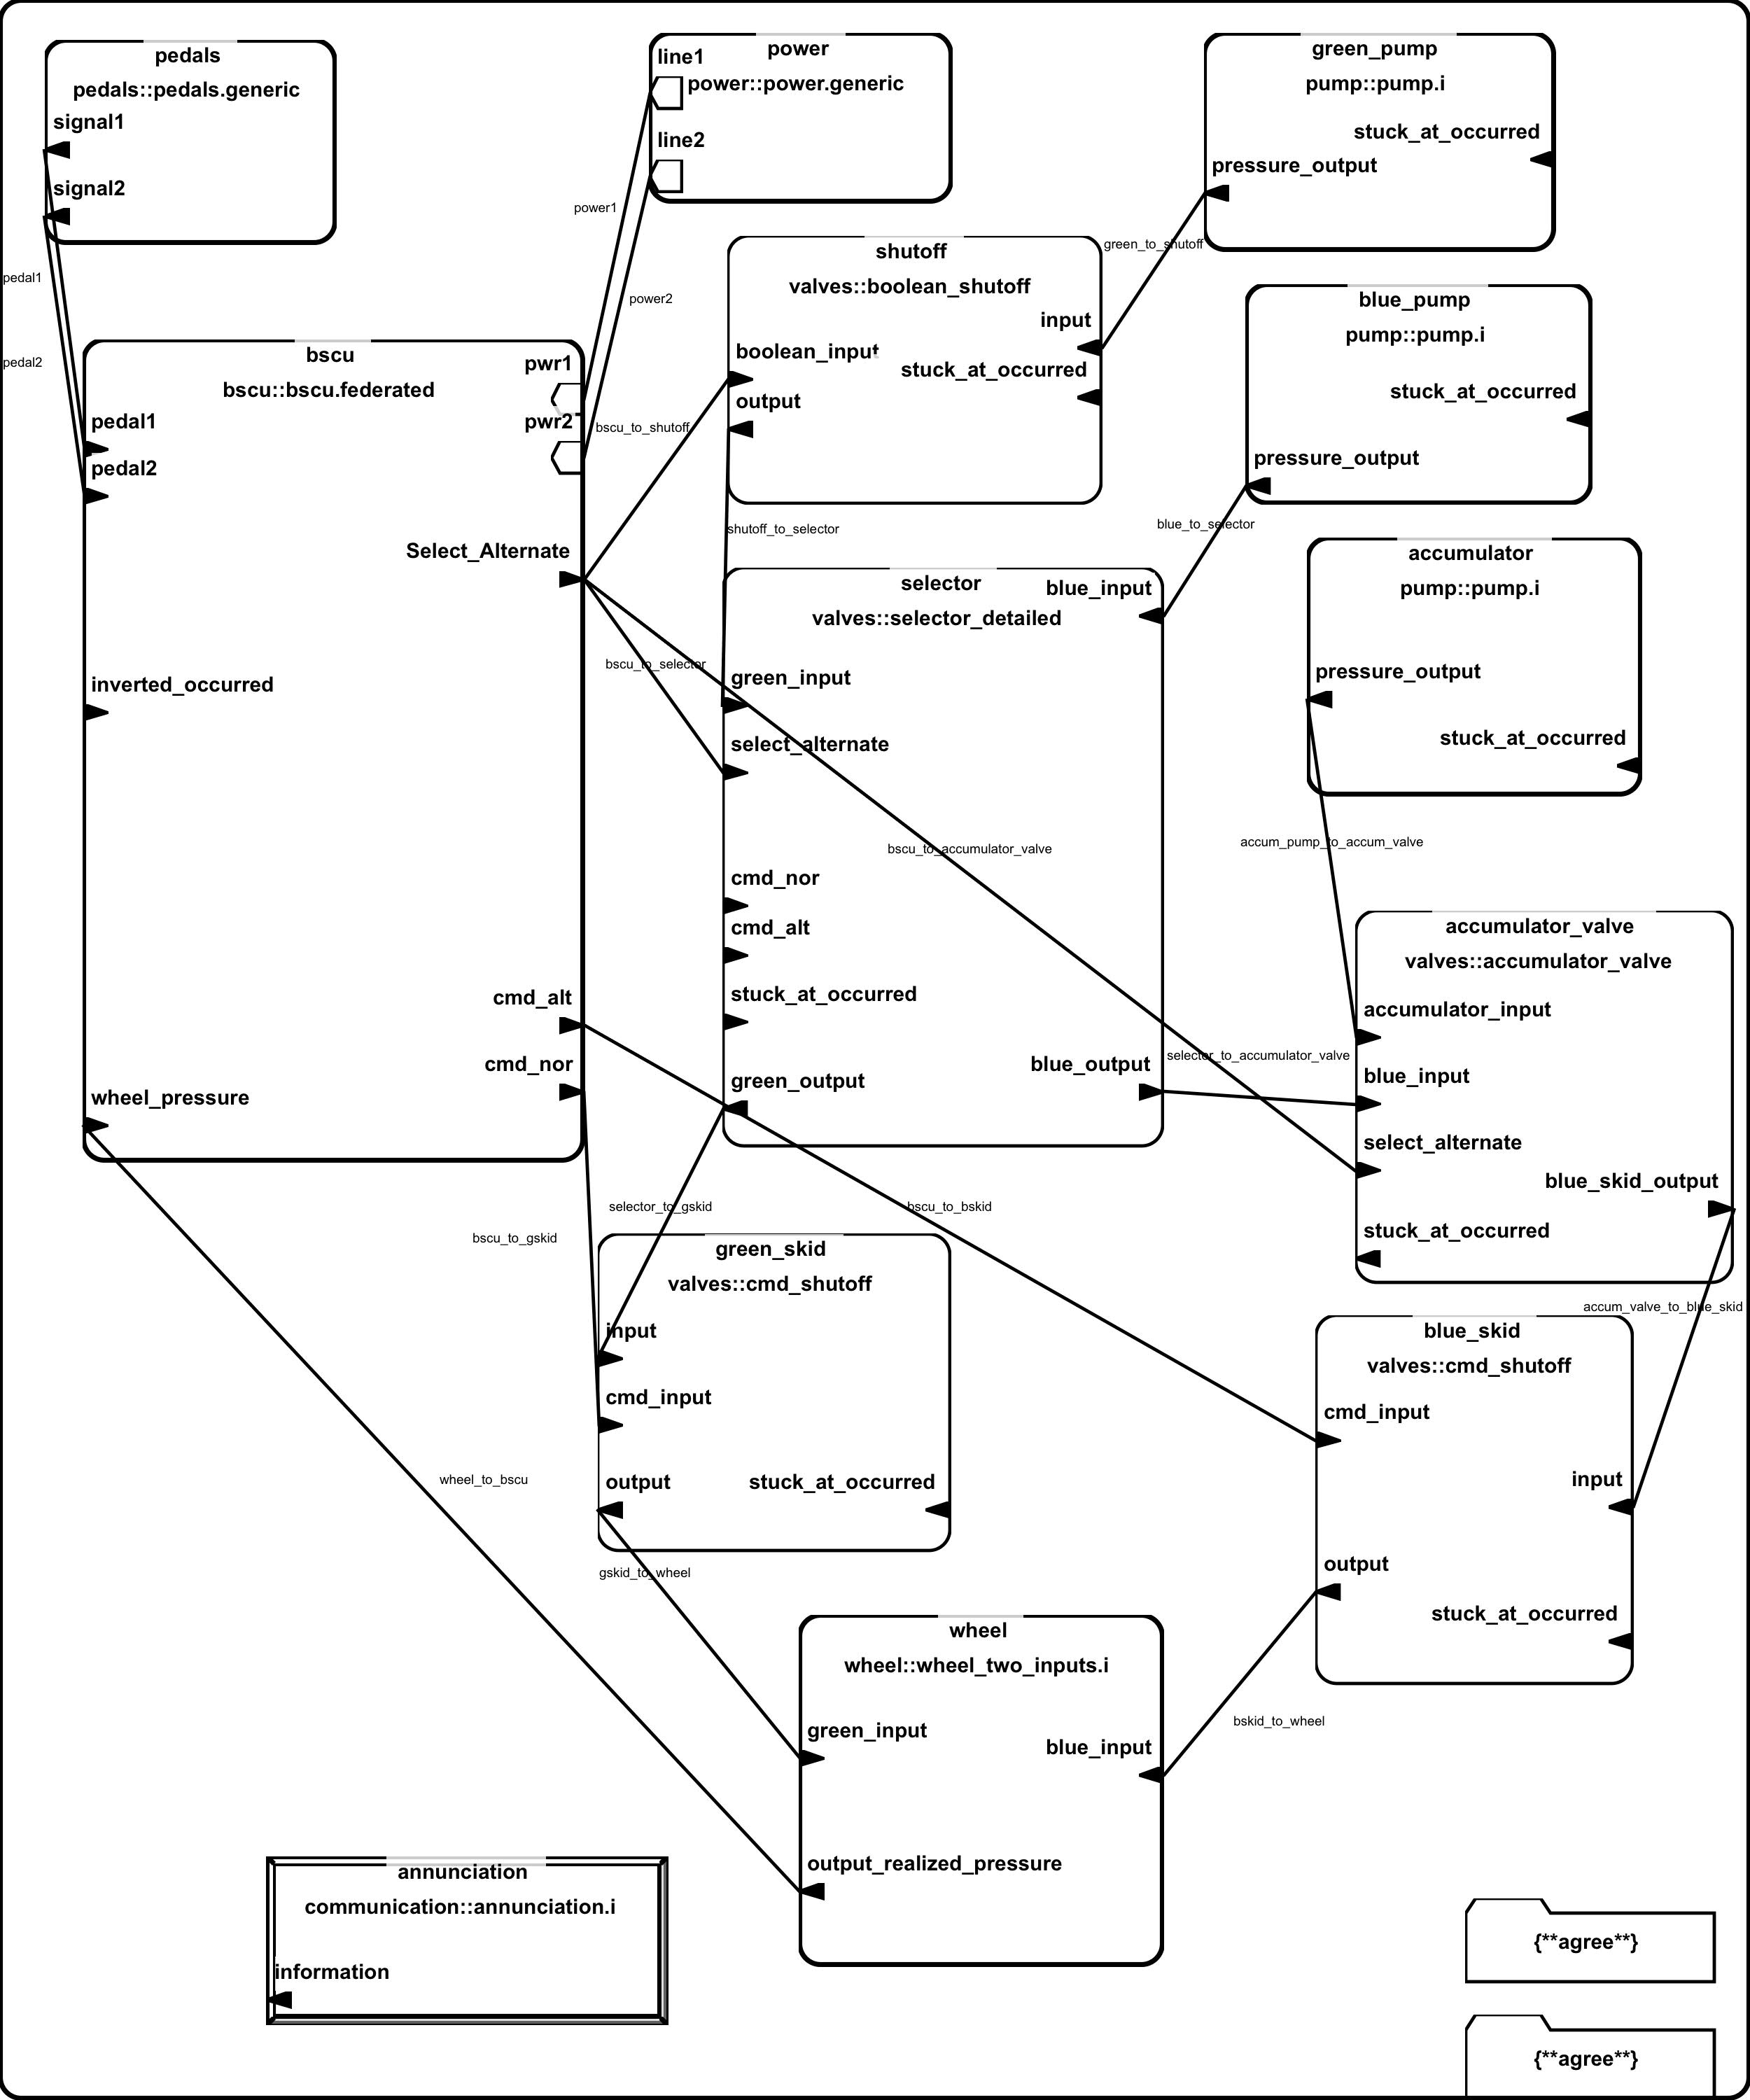
\includegraphics[width=\textwidth]{images/wbsfederated3.jpg}
\caption{AADL Simple Model of the Wheel Brake System }
\label{fig:wbs_ima}
\end{center}
\end{figure}

Each wheel has a brake assembly that can be operated by two independent hydraulic systems (designated green and blue). In normal braking mode, the green hydraulic system operates the brake assembly.  If there is a failure in the green hydraulics, the system switches to alternate mode which uses the blue hydraulic system.  The blue system is also supplied by an accumulator which is a device that stores hydraulic pressure that can be released if both of the primary hydraulic pumps (blue and green) fail. The accumulator supplies hydraulic pressure in Emergency braking mode.

Switching between the hydraulic pistons and pressure sources can be commanded automatically or manually. If the hydraulic pressure in the green supply is below a certain threshold, there is an automatic switchover to the blue hydraulic supply. If the blue hydraulic pump fails, then the accumulator is used to supply hydraulic pressure.

In both normal and alternate modes, an anti-skid capability is available. In the normal mode, the brake pedal position is electronically fed to a computer called the Braking System Control Unit (BSCU). The BSCU monitors signals that denote critical aircraft and system states to provide correct braking function, detect anomalies, broadcast warnings, and sent maintenance information to other systems.

\subsection{Nominal System Model}
\label{sec:nominal}
The WBS AADL model of the nominal system behavior consists of mechanical and digital components and their interconnections, as shown in Figure~\ref{fig:wbs_ima}. The following section describes this nominal model from which the fault model was generated.

\paragraph{Wheel Braking System (WBS)}
The highest level model component is the WBS. It consists of the BSCU, green and blue hydraulic pressure lines (supplied by the green pump  and blue pump/accumulator respectively), a Selector which selects between normal and alternate modes of hydraulic pressure, and the wheel system. The WBS takes inputs from the environment including PedalPos1, AutoBrake, DecRate, AC\_Speed, and Skid. All of these inputs are forwarded to the BSCU to compute the brake commands.

\paragraph{Braking System Control Unit (BSCU)}
The BSCU is the digital component in the system that receives inputs from the WBS. It also receives feedback from the green and blue hydraulic lines and two power inputs from two separate power sources. The BSCU is composed of two command and monitor subsystems each powered independently from separate power sources. The pedal position is provided to these units and when skidding occurs, the command and monitor units will decrease the pressure to the brakes.
The command unit regulates the pressure to the brakes in the green hydraulic line through the command cmd\_nor. Computing this command requires both the brake requested power and the skid information. The command unit also regulates the pressure in the blue hydraulic line in order to prevent skidding which it does through the cmd\_alt command. The monitor unit checks the validity of the command unit output.

The BSCU switches from normal to alternate mode (blue hydraulic system) when the output from either one of its command units is not valid or the green hydraulic pump is below its pressure threshold.  Once the system has switched into alternate mode, it will not switch back into normal mode again.

\paragraph{Hydraulic Pumps}
There are three hydraulic pumps in the system, green pump (normal mode), blue pump (alternate mode), and accumulator pump (emergency mode). Each pump provides pressure to the system and is modeled in AADL as a floating point value.

\paragraph{Shutoff Valve}

The shutoff valve is situated between the green pump and the selector. It receives an input from the BSCU regarding valve position and regulates the pressure coming through the green pipe accordingly.

\paragraph{Selector Valve}
The selector receives inputs from the pumps regarding pressure output and the BSCU regarding which mode the system is in. It will output the appropriate pressure from green, blue, or accumulator pump. An added requirement of the selector system is that it will only output pressure from one of these sources. Thus, the case of having pressure supplied to the wheels from more than one pump is avoided. The Selector takes the two pipe pressures (green and blue) as input, selects the system with adequate pressure and blocks the system with inadequate pressure. If both systems have pressure greater than the threshold, the AADL selects normal mode as the default.

\paragraph{Skid Valves}
The blue\_skid and green\_skid valves receive input from the selector as pressure coming through the respective pipes as well as input from the BSCU that commands normal or alternate mode. The skid valves will use these inputs to choose between the green or the blue pressure to send to the wheel.

\subsection{Modeling Nominal System Behavior}
In order to reason about behaviors of complex system architectures, we have developed a compositional verification tool for AADL models.
Our tool, the {\em Assume-Guarantee Reasoning Environment} (AGREE) \cite{NFM2012:CoGaMiWhLaLu}  is based on {\em assume-guarantee} contracts that can be added to AADL components.  The language used for contract specification is based on the LUSTRE dataflow language~\cite{Halbwachs91:IEEE}. The tool allows scaling of formal verification to large systems by splitting the analysis of a complex system architecture into a collection of verification tasks that correspond to the structure of the architecture.

We use AGREE to specify behavioral contracts corresponding to the behaviors expected of each of the WBS components. An example of a contract is shown in Figure~\ref{fig:agreeContract}.
%

\begin{figure}
\begin{center}
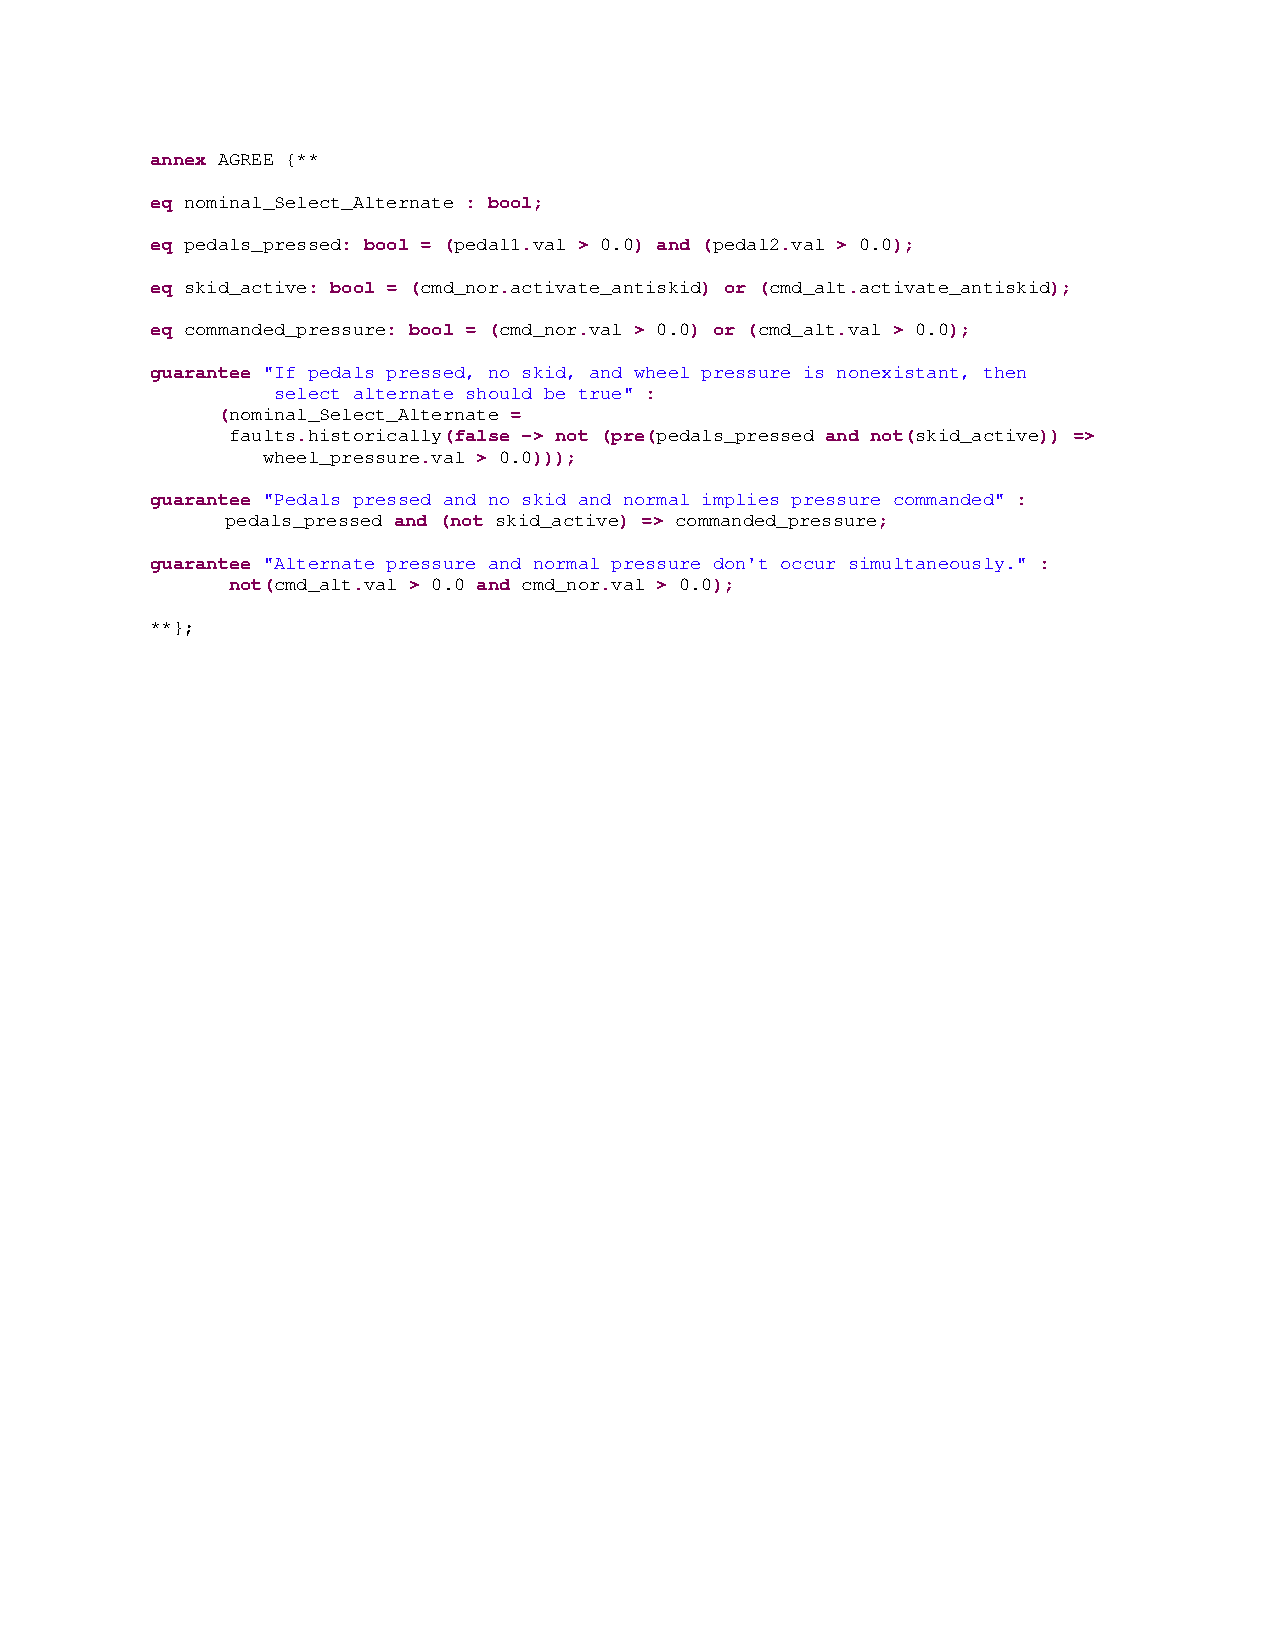
\includegraphics[trim=60 480 50 60,clip,width=\textwidth]{images/bscu.pdf}
\caption{AGREE Contract for BSCU }
\label{fig:agreeContract}
\end{center}
\end{figure}

\iffalse

\subsection{Nominal System Modeling}
\mike{KEEP HERE!}
A formal specification of the nominal system model consists of mechanical and digital components and their interconnections.

The highest level component is the Wheel Braking System (WBS). It consists of a digital control unit, the BSCU, and normal and alternate hydraulic pressure lines (supplied by green pump and blue pump/accumulator respectively). The system takes inputs from the environment including PedalPos1, AutoBrake, DecRate, AC\_Speed, and Skid. All of these inputs are forwarded to the BSCU to compute the brake commands. The outputs of the WBS are normal\_pressure, alternate\_pressure, and System\_Mode (normal, alternate, EMERGENCY).

\subsection{Braking System Control Unit (BSCU)}
The BSCU is the digital component in the system that receives inputs from the WBS. It also receives feedback from the normal and alternate lines and two power inputs from two separate power sources.

\fi



\section{Background}
This section provides a high level description of the pieces of the puzzle necessary in order to understand our approach. We describe the relevant algorithms and tools in order to make the later formalisms fit into the full picture. 

\subsection{Inductive Validity Cores}

Given a complex model, it is often useful to extract traceability information related to the proof, in other words, which portions of the model were necessary to construct the proof. An algorithm was introduced by Ghassabani, et. al. to provide Inductive Validity Cores (IVCs) as a way to determine which model elements are necessary for the inductive proofs of the safety properties for sequential systems~\cite{GhassabaniGW16}. Given a safety property of the system, a model checker can be invoked in order to construct a proof of the property. The IVC generation algorithm can extract traceability information from that proof process and return the model elements required in order to prove the property. A short time later, this algorithm was refined in order to produce the minimal set of such IVC elements~\cite{Ghassabani2017EfficientGO}. 

This algorithm is of interest to us for the following reason. By letting the negation of the safety property of interest be our top level event, we can utilize the algorithm to find the set of minimal IVCs which will tell us the minimal model elements (including faults) necessary to prove that this top level event occurs. In other words, we will know the minimal set of events required in order to cause the occurance of the top level event. These model elements consist of the active faults present in the system and the contracts of components that were effected by the presence of the fault. This gives a trace of how the fault propagates through system components and how the software behaves in the presence of the faults. 

In section III, we show the formal definitions of IVCs in detail. \\

Our approach utilizes a few tools in order to generate the artifacts of interest and a brief background will be helpful. and hence the rest of the background section consists of a brief description of AADL, AGREE, and the SOTERIA tools and languages. 

\subsection{Architecture Analysis and Design Language}
We are using the Architectural Analysis and Design Language (AADL)~\cite{FeilerModelBasedEngineering2012} to construct system architecture models.  AADL is an SAE International standard that defines a language and provides a unifying framework for describing the system architecture for ``performance-critical, embedded, real-time systems''~\cite{AADL_Standard}. From its conception, AADL has been designed for the design and construction of avionics systems.  Rather than being merely descriptive, AADL models can be made specific enough to support system-level code generation.  Thus, results from analyses conducted, including the new safety analysis proposed here, correspond to the system that will be built from the model.  

An AADL model describes a system in terms of a hierarchy of components and their interconnections, where each component can either represent a logical entity (e.g., application software functions, data) or a physical entity (e.g., buses, processors). An AADL model can be extended with language annexes to provide a richer set of modeling elements for various system design and analysis needs (e.g., performance-related characteristics, configuration settings, dynamic behaviors). The language definition is sufficiently rigorous to support formal analysis tools that allow for early phase error/fault detection.

\subsection{Compositional Analysis} Compositional analysis of systems was introduced in order to address the scalability of model checking large software systems. Monolithic verification and compositional verification are two ways that mathematical verification of component properties can be performed. In monolithic analysis, the model is flattened and the top level properties are proved using only the leaf level contracts of the components. On the other hand, the analysis can be performed compositionally following the architecture hierarchy such that analysis at a higher level is based on the components at the next lower level.  When compared to monolithic analysis (i.e., analysis of the flattened model composed of all components), the compositional approach allows the analysis to scale to much larger systems~\cite{NFM2012:CoGaMiWhLaLu}. 

\subsection{Assume Guarantee Reasoning Environment}
The Assume Guarantee Reasoning Environment (AGREE) is a tool for formal analysis of behaviors in AADL models~\cite{NFM2012:CoGaMiWhLaLu}.  It is implemented as an AADL annex and annotates AADL components with formal behavioral contracts. Each component's contracts can include assumptions and guarantees about the component's inputs and outputs respectively, as well as predicates describing how the state of the component evolves over time.

AGREE translates an AADL model and the behavioral contracts into Lustre~\cite{Halbwachs91:IEEE} and then queries a user-selected
model checker to conduct the back-end analysis. The analysis can be performed compositionally following the architecture hierarchy such that analysis at a higher level is based on the components at the next lower level.  When compared to monolithic analysis (i.e., analysis of the flattened model composed of all components), the compositional approach allows the analysis to scale to much larger systems~\cite{QFCS15:backes}. 

\subsection{Safety Annex for AADL}
The Safety Annex for AADL is a tool that provides the ability to reason about faults and faulty component behaviors in AADL models~\cite{Stewart17:IMBSA,SATechReport}. In the Safety Annex approach, formal assume-guarantee contracts are used to define the nominal behavior of system components. The nominal model is verified using AGREE. The Safety Annex weaves faults into the nominal model and analyzes the behavior of the system in the presence of faults. The tool supports behavioral specification of faults and their implicit propagation through behavioral relationships in the model as well as provides support to capture binding relationships between hardware and software compönents of the system. 

\subsection{SOTERIA}
The Safe and Optimal Techniques Enabling Recovery, Integrity, and Assurance (SOTERIA) tool is used to perform safety analysis of Integrated Modular Avionics (IMA) systems~\cite{SOTERIAproject}. In the SOTERIA project, a compositional modeling language was developed and this language is used as input in order to automatically synthesize the qualitative and quantitative safety analyses. The tool is compositional in that it requires safety aspects at each component level which enables the generation of compositional fault trees. 

\begin{figure}[h]
\begin{center}
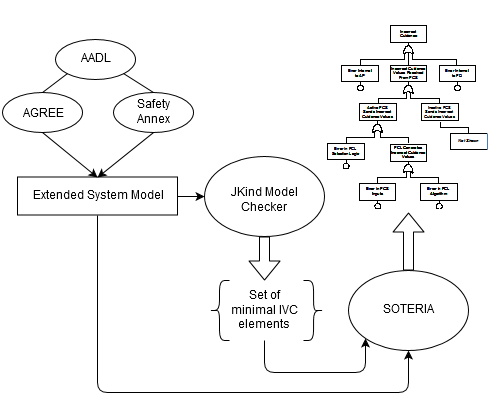
\includegraphics[width=8cm]{images/processFTA.png}
\caption{Outline of the fault tree generation process} \label{fig:processFTA}
\end{center}
\end{figure}

\subsection{Fault Tree Analysis} A Fault Tree (FT) is a directed acyclic graph whose leaves model component failures and whose gates model failure propagation. The system failure under examination is the root of the tree and is called the Top Level Event (TLE). The Basic Events (BE) are the events that can occur in the system which lead to the TLE and in the graphical model, these correspond to the leaves. Figure~\ref{fig:introFT} shows a simple example of a fault tree based on SAE ARP4761~\cite{SAE:ARP4761}. In this example, the top level event corresponds to an aircraft losing all wheel braking. In order for this event to occur, all of the basic events must occur. This is seen through the use of the AND gate below the top level event. The gates in the fault tree describe how failures propagate through the system. Each gate has one output and one or more inputs. In Figure~\ref{fig:introFT}, the AND gate has three inputs and one output. The leaves of the tree represent the basic events of the system and in the case of this fault tree, these three events are also the \textit{minimum cut set} for this top level event. The minimal cut set is the minimum set of basic events that must occur together in order to cause the TLE to occur. Finding these sets is important to FTA and has been an active area of interest in the research community since fault trees were first described in Bell Labs in 1961~\cite{historyFTA}. 

\begin{figure}[h]
\begin{center}
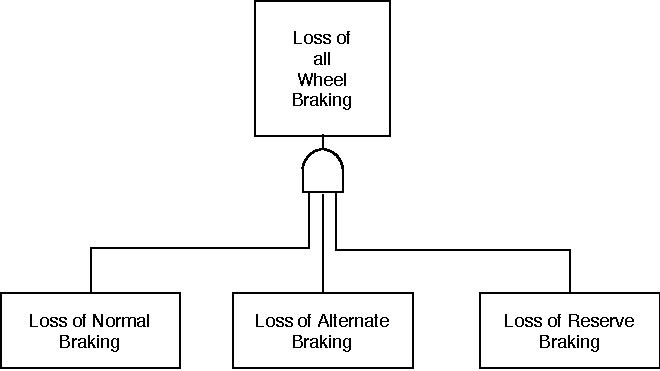
\includegraphics[width=8cm]{images/introFT2.pdf}
\caption{A simple fault tree} \label{fig:introFT}
\end{center}
\end{figure}

There are two main types of FTA that we differentiate here as \textit{qualitative} analysis and \textit{quantitative} analysis. In qualitative analysis, the structure of the fault tree is considered and the cut sets are a way to indicate which combinations of component failures will cause the system to fail. On the other hand, in quantitative analysis the probability of the TLE is calculated given the probability of occurance of the basic events. 

The formal definition of a fault tree is provided in section III and more details regarding quantitative and qualitative FTA is explained there as well. 

The general outline of our process is as follows and is shown in Figure~\ref{fig:processFTA} (Note: the fault tree shown in Figure~\ref{fig:processFTA} is generic and the text is irrelevant). The AADL system model is annotated with behavioral contracts using AGREE and then extended with faults using the Safety Annex. These three things together make the extended system model as shown in the figure. The extended system model is given to the JKind model checker~\cite{2017arXiv171201222G} which outputs the minimal sets of IVC elements for each layer of the architecture. These IVC elements and pertinant details of the extended system model is given to the SOTERIA tool whose output is the graphical fault tree representation of the input. 


%\section{New MBSA Capabilities}

\mike{REWRITE!}

Previous research has been based on MBD tools (such as Simulink and SCADE) that were available at the time \cite{Joshi05:Dasc}. However, these tools are really targeted at the design and implementation of software components, rather than at the system architecture level where most safety concerns arise.

Within the past five years there have been great advances in the capabilities of tools for modeling and analysis of at the system level, based on languages such as SysML \cite{SysML} and AADL \cite{AADL}. We use these new MBSE capabilities and extend them to implement the safety analysis methods needed for the design and certification of commercial aircraft systems. The system modeling tools that we plan to use are based on AADL, but they can import and export models from SysML.

\begin{itemize}
\item We will improve the efficiency of MBSA methods by using MBSE tools that can perform compositional reasoning over complex system models. Using the assume- guarantee contract mechanism, these tools provide support for heterogeneous component models implemented in different languages (such as Simulink or C/C++).

\item Our new analysis methods move away from traditional static safety analysis methods focused on probabilistic models (e.g., Fault Tree Analysis), to the direct modeling of potential failure mechanisms and the analysis of dynamic fault-mitigation strategies.

\item Formal verification of system models provides increased assurance that these models are accurate and will produce correct results. The hierarchical structure of system architecture models supports analysis at varying levels of abstraction. Compositional analysis explicitly checks assumptions captured in component and subsystem contracts. Consistency and realizability checks [23] provide the ability to detect conflicting requirements between component and subsystem models.
\end{itemize}

%In this section we describe some of the new capabilities that we will develop, including improvements related to the AADL Error Model Annex, the use of model-based assurance cases, and evaluation of system-level certification objectives related to system safety that can be satisfied using the proposed methods.
\danielle{Removed the sections that were written in the safety.tex portion of the paper.}
%We bridge the descriptions of errors in the error model annex with behavioral descriptions of components. We start from the error model notions of error types and state machines that describe transitions from nominal to error states. However, we then tie these nominal and error states to behavioral models of the components in question that describe how the faults manifest themselves in terms of the signals or quantities produced by the components. Now the behavioral models can provide implicit propagation of the faulty behaviors and the natural consequences of failures on component behavior will be manifested in the propagation of other component faults through the behavioral model.

%To accomplish this, we use AADL and the error model annex to describe faults, and to use the AGREE contract specification language to describe behavioral models. This requires extensions to AGREE to define fault models that describe how different faults manifest themselves in changes to output signals. It also requires changes to the error annex. The conditions under which faults occur will become richer such that they describe not just propagation of enumerations from other components, but also valuations of input signals.





%\subsection{Fault and Behavioral Modeling}



\section{Architectural Failure Effect Modeling for the WBS}

We illustrate our FEM approach on the Wheel Braking System.  Starting from the nominal model described in Section~\ref{sec:nominal}, we first determine whether a given safety property of interest holds on a fault-free instance of the model.  We then extend the model with faults and determine whether the property continues to hold under reasonable fault scenarios.

The initial safety property to be proven determines whether the system will apply pressure to the wheels when commanded to do so:

\begin{tt}
\  \\
If pedals are pressed and no skid occurs, then the brakes will receive pressure. \\
\end{tt}

\noindent Using the reference AADL model constructed by the SEI~\cite{SEI:AADL} extended with AGREE contracts describing system behaviors, this property proves immediately.  From this point, we focus our attention on component failures and how this will affect the top level property of the system.

We would like to specify different component failure modes. These failure modes can be triggered by some internal or propagated fault. In order to trigger these faults, additional input was added to the AADL model for each fault that can occur within a nominal model component. This consists of two types:

\begin{itemize}
\item \textit{fail\_to} fault: This type of fault accounts for both nondeterministic failures and stuck-at failures. The components that are affected by this fault include meter valves and pumps. This fault can be used to describe both digital and mechanical errors. Examples of digital failures include a \textit{stuck\_at} failure for the command subsystem in the BSCU component, which causes the command unit to become stuck at a previous value. An example of a mechanical failure would be a valve stuck open (or closed).


\item \textit{inverted\_fail} fault: This type of fault will be used on components which contain boolean output. It will simply take boolean input, negate it, and output the negated value. An example of this is the selector. In the nominal model, input to the selector consists of a boolean value \textit{select\_alternate} value from the BSCU.

\end{itemize}

\begin{figure}[h!]
  \centering
 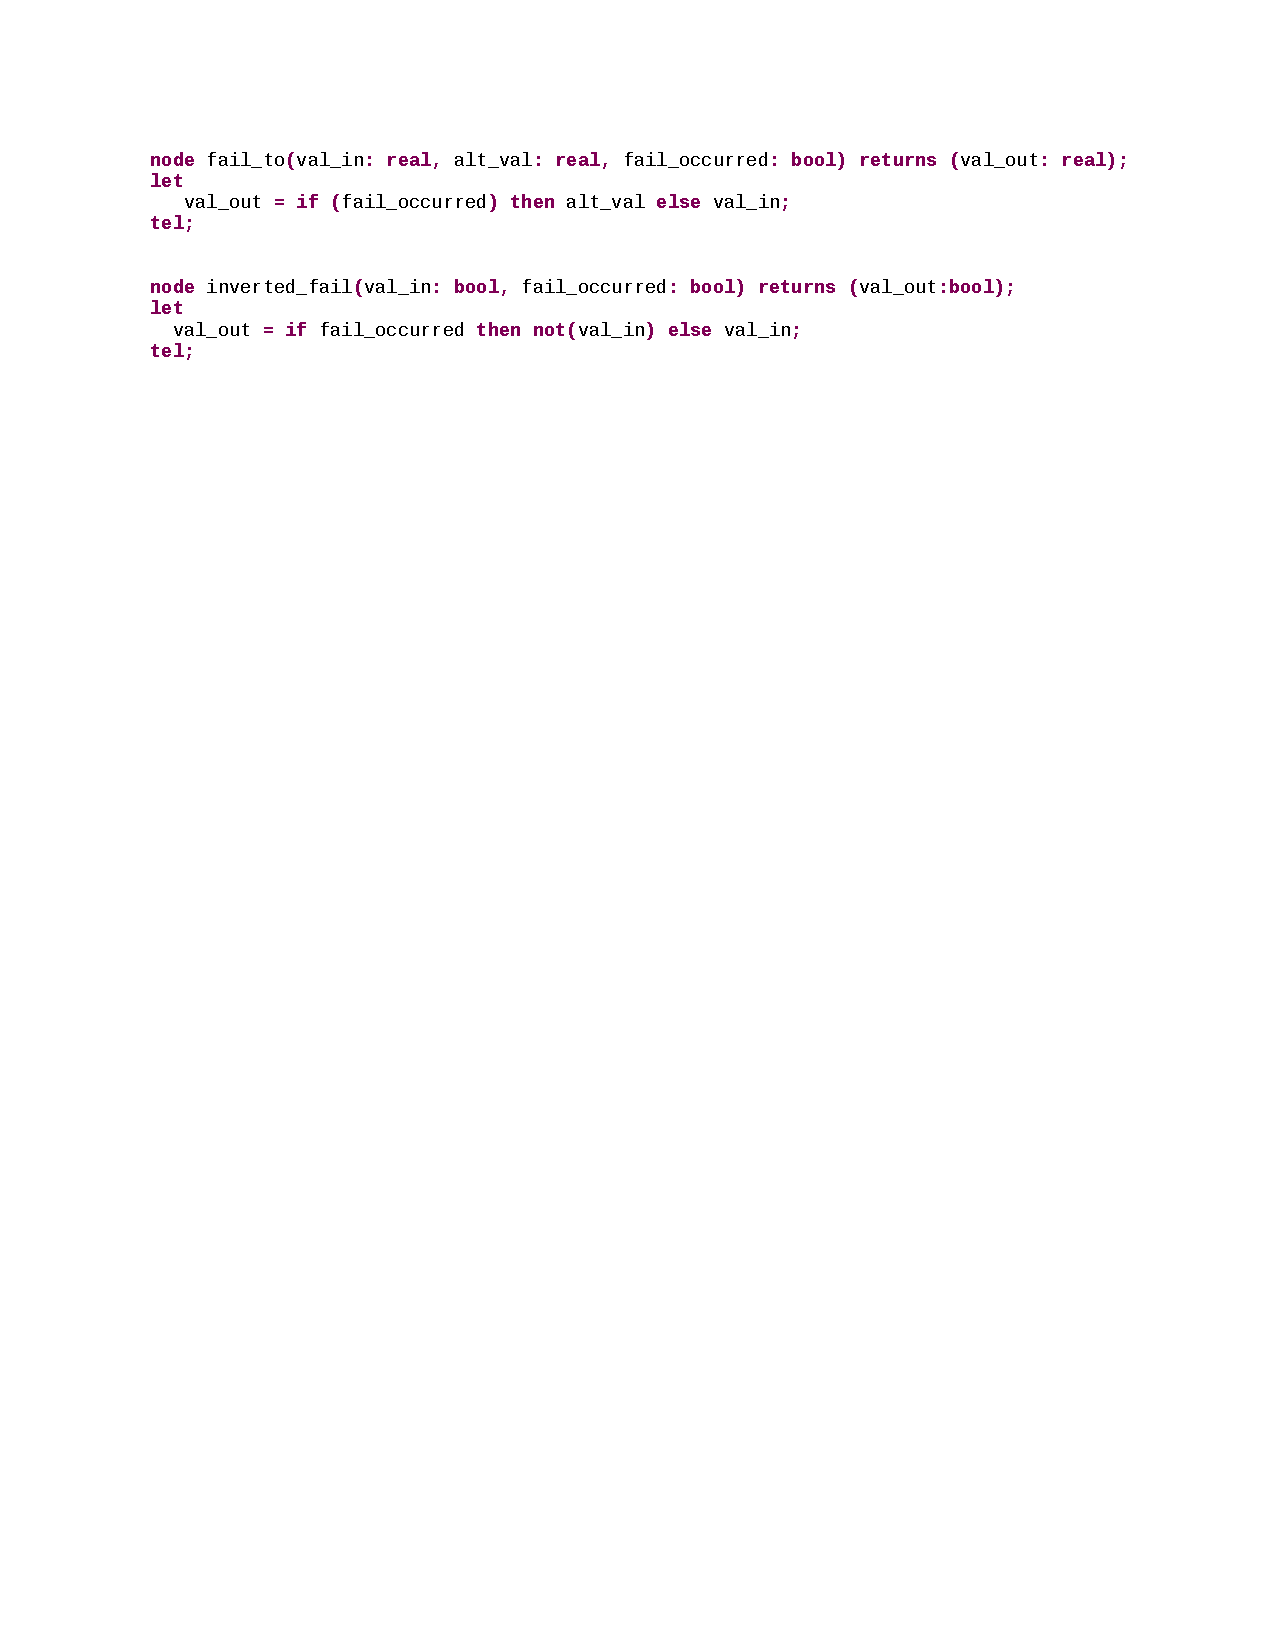
\includegraphics[trim=70 630 60 20,clip,width=1\textwidth]{images/fail_nodes.pdf}
  \vspace{-0.1in}
  \caption{AGREE Definition of a \textit{fail\_to} and \textit{inverted\_failure} Faults}
  \label{fig:failureNodes}
\end{figure}

These faults can be easily encoded in AGREE as shown in Figure~\ref{fig:failureNodes}.  The failures simply return an alternate value (for {\em fail\_to}) or invert the input value (for {\em inverted\_failure}) when a failure occurs.


While modeling faults, the duration of the fault must also be taken into account.  The AGREE tools allow a great deal of flexibility in terms of how faults are defined and their duration.  For the purposes of this model, we currently consider only {\em transient} and {\em permanent} faults, where transient faults occur for an instant in time (e.g., a single-event upset) and a permanent fault persists for the remainder of the system execution.


\subsection{Analysis of Faulty Models}
The following is a short summary of the failures defined in the fault model.

\begin{itemize}

\item Valves and Pumps: All valves and pumps have the possibility of a \textit{fail\_to} fault. This includes green pump, blue pump, accumulator, and the shutoff valves.

\item  The selector can also have a digital \textit{fail\_to} fault regarding the inputs from BSCU commanding to use normal or alternate means of pressure along with an \textit{inverted\_fail} fault which would change the boolean value that commands antiskid to activate.

\end{itemize}

Given our understanding of the WBS, our assumption was that any single permanent fault could be introduced into the system and the pilot would still be able to command brake pressure.  However, our analysis tools returned a counterexample to the property, and upon examination, the structure of the reference model was insufficient to guarantee the property.

%\subsection{Strengthening the Nominal Model}
The first issue was {\em feedback}; the reference model did not have a sensor to determine pressure after the selector valve.  This means that a single failure of (for example) the blue or green antiskid valve cannot be detected by the BSCU (see Figure~\ref{fig:wbs_ima}), and it cannot route around the failure.  In order to address this, we added a pressure sensor to the wheel that communicates with the BSCU to detect lack of pressure at the wheel.


After adding a sensing apparatus to the wheel, the analysis generated another counterexample due to a single failure of the selector valve.  In the reference model, there is a single selector component that takes as inputs the green pump, the blue pump, and the accumulator.  A single failure in this component can lead to no pressure along either of the two outgoing pressure lines.
To solve this issue, we removed the accumulator from the selector and added an accumulator valve.   This component takes in the blue pressure from the selector and the accumulator pressure. It also takes in a \textit{select\_alternate} flag from the BSCU. The output of the accumulator\_valve goes directly to the blue\_skid component and is either the blue or the accumulator pressure.

Finally, our BSCU is currently structured to always fail-over from the green system to the blue system but never the reverse.  Because of this choice (which matches the AIR6110 document), it is also necessary to guarantee that \textit{select\_alternate} is false until a failure occurs in the system; otherwise, a single failure in the blue anti-skid valve can cause the system to fail to provide pressure.  This asymmetry is something that could be revisited in future work.


Even after making these three changes to the model, the original property still does not prove.  At issue is that the sensing of a no-pressure situation is not instantaneous; there is a delay for this information to reach the BSCU and be acted upon to switch to the alternate braking system.  In our current timing model for the system, the feedback to the BSCU involves a delay, but the BSCU and valves can react.  Thus, we weaken our top-level property to state that if the brakes are pressed for two consecutive time instants, then pressure will be provided to the wheels:

\begin{tt}
\ \\
If pedals are pressed in the previous state and pressed in the current state and no skid occurs, then the brakes will receive pressure. \\
\end{tt}

The nominal WBS model extended with the faults described in this section can be found at \textit{https://github.com/loonwerks/AMASE}. 


















\section{Discussion}
We have used the WBS model as a vehicle to experiment with different modeling and fault representation ideas, and to get a feel for the scalability of our approach.
%
We started from the reference AADL model~\cite{SEI:AADL} to attempt to contrast our FEM approach using AGREE contracts vs. the FLM-based approach that was already part of this model.  Part of this was driven by curiosity as to whether important faults might be caught by one approach and missed by the other, and to contrast the two styles of analysis.

During the process of defining and injecting faults, subtle issues of the system structure and behavioral interactions became much clearer.  The idea that the system must use the green side until a failure occurs was unexpected.  In addition, the extensions to the model were driven by the counterexamples returned by the tools.   The approach quickly and precisely provided feedback towards aspects of the system that were not robust to failure.  The researcher who produced the model (Stewart) was not involved in earlier MBSA work and had no prior exposure to the WBS model and yet was able to relatively quickly construct a fault-tolerant model.  The fact that these holes in the reference model perhaps means that the behavioral approach can be better at drawing attention to certain kinds of failures.

On the other hand, the utility of the safety analysis is driven by the ``goodness'' of the properties.  Our one example property is clearly insufficient: for example, it is not possible to detect faults related to over-pressurization or misapplication of the brakes when no braking is commanded.  Of course, any complete analysis should have properties related to each hazardous condition.  The approach is foundationally a top-down analysis (like fault trees) rather than a bottom up approach (like a FMEA / FMECA).  In addition, if properties are mis-specified, or the system dynamics are incorrectly modeled, then properties may verify even when systems are unsafe.  The explicit propagation approach of the FLM techniques force the analyst to consider each fault interaction.  This too is a double-edged sword: when examining some of the fault propagations in the reference model, we disagreed with some of the choices made, particularly with respect to the selector valve.  For example, if no select alternate commands are received from the BSCU, then both the green and blue lines emit a {\em No\_Service} failure.

In terms of scalability, the analysis time for counterexamples was on the order of 1-2 seconds, and the time for proofs was around 4 seconds, even after annotating the model with several different failures.  From earlier experience applying compositional verification with the AGREE tools (e.g.,~\cite{QFCS15:backes,hilt2013}), we believe that the analysis will scale well to reasonably large models with many component failures, but this will be determined in future work.

The analysis in this paper involved hand-annotating the models with failure nodes.  This process is both schematic and straightforward: we define the AGREE contracts over internal {\em nominal output variables} and then define the actual outputs using the nominal output variables as inputs to the fault nodes like those in Figure~\ref{fig:failureNodes}.   We are currently in the process of defining a fault integration language which will eliminate the need for hand-annotation.  Some aspects of the Error Annex could be directly relevant: the state machines describing leaf-level faults could easily be compiled into behavioral state machines that determine when faults occur.  On the other hand, in a behavioral approach we need to be able to bring in additional quantities (inputs, parameters) to instantiate behavioral faults, and the two approaches have very different notions of propagation.

The xSAP tool~\cite{DBLP:conf/tacas/BittnerBCCGGMMZ16} has an elegant extension language that allows for fault definition, selection between multiple faults for a component, and ``global'' dependent faults that can affect multiple components.  The authors have used this support to construct a sophisticated analysis model for the WBS~\cite{DBLP:conf/cav/BozzanoCPJKPRT15}.  However, some useful aspects of fault modeling, such as global faults that are driven by the state of the model, appear to be hard to construct.  For example, a pipe-burst failure can be seen as a global failure because it may cause unconnected components within the model to fail, so can be represented as having a certain probability.  On the other hand, the likelihood of failure in the real system is driven by the number of currently pressurized pipes in the system, which appears to be hard to define.  We hope to allow for such conditional and model-driven failures in our fault definition language.





\section{Conclusion}
\label{sec:conclusion}
We have developed an extension to the \gls{aadl} language with tool support for formal analysis of system safety properties in the presence of faults. The nominal model is extended with fault definitions, which allows safety analysis and system implementation to be driven from a single common model. The use of formal methods supports comprehensive exploration on the effect of faulty component behaviors on the system level failure condition without the need to add separate propagation specifications to the model. During the development of this approach we worked closely with safety engineers to ensure that the needs of the analysts are supported. This approach was illustrated through the use case of an aircraft system, but can be applied on the development of critical systems in multiple domains. 

The contributions described in this paper are as follows:

\begin{itemize}
\renewcommand{\labelitemi}{\textbullet}
		\item close integration of behavioral fault analysis into \gls{aadl}, which allows close connection between system and safety analysis and system generation from the model,
		\item support for behavioral specification of faults and their  implicit propagation through behavioral relationships in the model,
		\item additional support to capture binding relationships between hardware and software and logical and physical communications, %and
		\item the use of formal methods to automatically verify safety properties in the presence of faults and comprehensively enumerate all applicable fault combinations leading to failure conditions under quantitative objectives as part of the safety assessment process, and
		\item guidance on integration into a traditional safety analysis process.
\end{itemize}

Future work includes compilation of minimal cut sets into graphical fault tree format, expanding the user interface to provide ease in fault model creation, and transforming the counterexample into a sequence flow showing how the system changes as faults are activated. The research presented in this paper, as well as the contributions of future work, all serve to support the safety assessment process. These contributions do not encompass all of the assessment process, but instead aim to provide automated and comprehensive analysis and also to generate evidence for the assessment process.



\vspace{2 mm}
\noindent {\bf Acknowledgments.} This research was funded by NASA contract NNL16AB07T and the University of Minnesota College of Science and Engineering Graduate Fellowship.


%ACKNOWLEDGMENTS are optional
%TODO: Fill in for final version
\vspace{0.08in}


%\textbf{Acknowledgments:}
%This work was supported by

%We thank XXXX

\bibliographystyle{abbrv}
\bibliography{biblio}

% This ~ seems to fix an odd bibliography alignment issue
~

%\ifdefined\TECHREPORT
%\appendix
%
%\section{Appendix: Proof of Equivalence}
%\input{appendix}
%\fi

%\section{Appendix: GPCA CENTA Model}
%\label{appendix:gpcacenta}
%\begin{figure}[!ht]
%\begin{center}
%\includegraphics[scale=0.6]{images/sampled_pca.PNG} %[trim = 0 2 0 0, clip=true]{Comp}
%\caption{GPCA AGREE Properties modeled as a Timed Automata} \label{fig:samplepca}
%\end{center}
%\end{figure}

%\balancecolumns

\end{document}
